

\documentclass[8pt, usepdftitle=false]{beamer}


% \imput{../common/beamerthemesimple}
\usetheme{simple}


  \usepackage{xcolor}
  \definecolor{olive}{rgb}{0.3, 0.4, .1}
  \setbeamercolor{itemize/enumerate body}{fg=black}
  \setbeamercolor{title}{fg = green!30!black}
  \setbeamercolor{frametitle}{fg = gray!70!black, bg = white}


% \usepackage{lmodern}
\usepackage[scale = 2]{ccicons}
\usepackage[export]{adjustbox}
\usepackage{amsmath, amsthm, amssymb}
\usepackage{amsfonts}
\usepackage{mathtools}

\usepackage[justification=raggedright,width=\linewidth]{caption}
\usepackage{tikz} 


\usepackage{setspace}

\setbeamertemplate{title page}[default][right,colsep=-4bp,rounded=true,shadow=\beamer@themerounded@shadow]

\setbeamertemplate{caption}[numbered]


%% Options

\setbeamercolor{alerted text}{fg=blue}
\setbeamertemplate{alerted text begin}{\itshape}
\setbeamertemplate{alerted text end}{}

\newenvironment<>{varblock}[2][\textwidth]{%
    \setlength{\textwidth}{#1}
    \begin{actionenv}#3%
        \def\insertblocktitle{\underline{#2}}%
        \par%
        \usebeamertemplate{block begin}}
        {\par%
        \usebeamertemplate{block end}%
    \end{actionenv}}

\setbeamertemplate{blocks}[rounded][shadow=true]
\setbeamercolor{block title}{fg=black,bg=gray!20!white}
\setbeamercolor{block body}{fg=black,bg=gray!10!white}




%% Theorem

% \newtheorem{theorem}{Theorem}

%% Bangla tex


\usepackage{polyglossia}
\setotherlanguage[numerals=Devanagari]{bengali}
\setmainlanguage{english}
\newfontfamily\bengalifont[Script=Bengali]{Akaash}


%% tikx

\usepackage{tikz}
\usetikzlibrary{calc,trees,positioning,arrows,fit,shapes,calc}





\newcommand\blfootnote[1]{%
  \begingroup
  \renewcommand\thefootnote{}\footnote{#1}%
  \addtocounter{footnote}{-1}%
  \endgroup
}



\newcommand\Permute[2][^n]{\prescript{#1\mkern-2.5mu}{}P_{#2}}
\newcommand\Combine[2][^n]{\prescript{#1\mkern-0.5mu}{}C_{#2}}


\renewcommand*{\thefootnote}{\fnsymbol{footnote}}


\usepackage{flexisym}
\usepackage{breqn}

\usepackage[T1]{fontenc}

% \usepackage{mathpazo}
% \renewcommand{\rmdefault}{put}

% \usepackage{fourier} 
% Only use the math font of mathpazo
% \let\temp\rmdefault
% \usepackage{mathpazo}
% \let\rmdefault\temp
% \renewcommand{\rmdefault}{put}


% \usepackage[hyphens]{url}


  % \usefonttheme{professionalfonts} % using non standard fonts for beamer
  % \usefonttheme{serif} % default family is serif

  % \usepackage{gentium}
  \usepackage{multicol}
  \usepackage{mathpazo}



% \renewcommand{\familydefault}{\sfdefault}  


  % color brackets
  \makeatletter
  \newcount\bracketnum
  \newcommand\makecolorlist[1]{%
      \bracketnum0\relax
      \makecolorlist@#1,.%
      \bracketnum0\relax
  }
  \def\makecolorlist@#1,{%
      \advance\bracketnum1\relax
      \expandafter\def\csname bracketcolor\the\bracketnum\endcsname{\color{#1}}%
      \@ifnextchar.{\@gobble}{\makecolorlist@}%
  }
  \let\oldleft\left
  \let\oldright\right
  \def\left#1{%
      \global\advance\bracketnum1\relax 
      \colorlet{temp}{.}%
      \csname bracketcolor\the\bracketnum\endcsname
      \oldleft#1%
      \color{temp}%
  }
  \def\right#1{%
      \colorlet{temp}{.}%
      \csname bracketcolor\the\bracketnum\endcsname
      \oldright#1%
      \global\advance\bracketnum-1\relax
      \color{temp}%
  }
  \makeatother


  \makecolorlist{black,blue,red}






\setbeamertemplate{section in toc}{%
  {\color{firstcolor}\inserttocsectionnumber.}~\inserttocsection}
\setbeamercolor{subsection in toc}{bg=white,fg=black}
\setbeamertemplate{subsection in toc}{%
  \hspace{1.2em}{\color{firstcolor}\rule[0.3ex]{3pt}{3pt}}~\inserttocsubsection\par}


\setbeamerfont{section in toc}{size=\fontsize{6}{8}\selectfont}
\setbeamerfont{subsection in toc}{size=\fontsize{6}{8}\selectfont}
\setbeamerfont{subsection in toc shaded}{size=\fontsize{6}{8}\selectfont}


\makeatletter
\patchcmd{\beamer@sectionintoc}{\vskip1.5em}{\vskip0.5em}{}{}
\makeatother






  \usepackage{twemojis}
  \usepackage{fontspec}
  \usepackage{tikzsymbols}
  \newfontfamily\DejaSans{DejaVu Sans}

% for R
\usepackage[fixed]{fontawesome5}


\setbeamercolor{emph}{fg=red}
\renewcommand<>{\emph}[1]{%
  {\color{purple}\only#2{\rm\itshape}#1}%
}

\setbeamertemplate{frametitle continuation}{}


\usepackage[round,  maxcitenames=10, mincitenames=11]{natbib}
\setlength{\bibhang}{0pt}
\renewcommand{\bibsection}{}
\usepackage{fancybox}


\setbeamertemplate{section page}
{
    \begingroup
    \begin{beamercolorbox}[sep=12pt,center]{section title}
        \usebeamerfont{section title}\insertsection\par
    \end{beamercolorbox}
    \endgroup
}

\setbeamertemplate{subsection page}
{
    \begingroup
    \begin{beamercolorbox}[sep=12pt,center]{section title}
        \usebeamerfont{section title}\insertsection\par
    \end{beamercolorbox}
    \vspace*{-1pt}
    \begin{beamercolorbox}[sep=8pt,center]{subsection title}
        \usebeamerfont{subsection title}\insertsubsection\par
    \end{beamercolorbox}
    \endgroup
}



\newcommand\Var[1]{\mathbb{V}\mathrm{ar}{#1}}



\renewcommand{\emph}[1]{%
{\rm\itshape{\color{purple}#1}}%
}

\renewcommand{\alert}[1]{%
{\rm\itshape{\color{blue}#1}}%
}

\newcounter{mytheorem}
\renewcommand{\themytheorem}{5.\arabic{mytheorem}}
\newcommand{\Thm}[1]{\refstepcounter{mytheorem}\textbf{#1\color{blue}\themytheorem}:}




%================ Give the title ============================##

\title{\LARGE Ch5 - Sampling Distribution}

\subtitle{{\fontsize{10}{10}\selectfont\color{gray!50!balck} 
(Sampling Dist. of Means and Proportions)} 
\\\vspace*{.2cm} Statistics For Business and Economics - I}

\author{Shaikh Tanvir Hossain\vspace*{-.4cm}}
\institute{ East West University, Dhaka\\ Last Updated \today}
\date{\vspace{-5pt}}
% \titlegraphic{\includegraphics[width=300,height=.5\textheight]{Images/EWU.png}}

% \setbeamertemplate{background}{\tikz[overlay,remember picture]\node[opacity=0.90]at (current page){\includegraphics[width=.5\textwidth,left]{EWU.png}};}


\usepackage{hyperref}
\hypersetup{
      pdftitle={Ch5 - Sampling Distribution},
        pdfauthor={Shaikh Tanvir Hossain},
          pdfborder={0 0 0},
       colorlinks,
      citecolor=blue,
      linkcolor=gray!50!black,
    breaklinks=true}




\begin{document}



% input the outline 

\begin{frame}[plain,noframenumbering] 
    \maketitle
\end{frame}
\setbeamertemplate{background}{}
\setlength{\abovedisplayskip}{-2pt}
\setlength{\belowdisplayskip}{4pt}
\setlength{\abovedisplayshortskip}{-3pt}
\setlength{\belowdisplayshortskip}{4pt}


\AtBeginSection[]
{
    \begin{frame}[plain, allowframebreaks]
\setstretch{.1}

        \setlength{\parskip}{1ex}
            \tableofcontents[sections={1-7}, 
            currentsubsection, 
            sectionstyle=show/hide, 
            sectionstyle=show/shaded, 
            ]
    \end{frame}
}


% Hide progress bar and footline on titlepage
\begin{frame}{Outline}
 \vspace*{.2cm}

\begin{center}
\begin{minipage}{10cm}
  \begin{alertblock}{Outline}
  \setstretch{.1}
   \setlength{\parskip}{1ex}
  \tableofcontents[sections={1-10}]
  %   \framebreak
  % \tableofcontents[sections={2}]
\end{alertblock}
\end{minipage}
\end{center}


\end{frame}



\begin{frame}[allowframebreaks]{}

\begin{itemize}
\item In this chapter we will see what happens when we do sampling. The important thing to always remember is that our sample itself is a random object. So anything that we can calculate from the sample is also random. Random objects that we calculate from the sample is generally called \emph{Sample Statistic} (it's a function of the random sample). For example, sample mean, sample proportion are all examples of sample statistics. 

\item When a sample Statistic targets a population parameter we call it an \emph{Estimator}. It's important that in real life we will never know the true population parameter. But we can use a sample an an estimator to estimate the population parameter. 


\item In \emph{repeated sampling}, the probability distribution of a sample statistic or the probability distribution of an estimator is called \emph{Sampling Distribution}. 

\item  The idea of Sampling Distribution is very important and almost like THE fundamental topic Statistics. It helps us to asses the variability of the sample statistic. 


\item So let's start...\faWalking \faWalking \faWalking.

\end{itemize}

\end{frame}



\section{Sample, Population and Statistical Inference}
\frame{\sectionpage}


\subsection{1. Sample and Random Sample}
\frame{\subsectionpage}


\begin{frame}[allowframebreaks]{Sampling}{finite and infinite population}

\begin{itemize}
 

   \item Consider following data (we saw this before), recall this was collected \emph{randomly} from $5$ students studying currently at EWU (hypothetical data). You know that the columns are called \alert{variables} and the rows are called \alert{observations} or \alert{units}.

      \medskip
      \begin{tabular}{l|c|c|c|c}
      \hline
       & Gender & Monthly Income (tk) & ECO-101 Grade & \# Retakes\\
      \hline
      Student 1. & Male & 3615 & B- & 3\\
      \hline
      Student 2. & Female & 49755 & A & 2\\
      \hline
      Student 3. & Male & 44758 & A & 1\\
      \hline
      Student 4. & Female & 3879 & B & 0\\
      \hline
      Student 5. & Male & 22579 & A+ & 2 \\
      \hline
      \end{tabular}

\bigskip
  \item This is \alert{a sample} right? Ques - 

    \begin{itemize}
        \item[]   What is \alert{the population} of this study? Ans - Everyone currently studying at EWU. 
    \end{itemize}

  \item Probability Theory was about modeling the population, recall we talked about population mean, population variance.  

  \item Now we will start \emph{Statistics} and \emph{Statistics starts from Sample} or more appropriately \emph{Random Sample}.

\framebreak

    \item What is a random sample? 

    \begin{itemize}
        \item    Is this particular sample random? Ans - NO, because we know all values.

        \item  Can we think about \emph{a sample which is random}? Ans - YES, 

        \item How? Think about \emph{repeated sampling} (or taking samples again and again and then the sample values will be random right?).
    \end{itemize}

    \item When we are thinking about repeated sampling, we can think the sample is actually a random object, since every-time we take a new sample, we will get different values.

    \item And that random object is what we will call a \alert{``a random sample''}. 

    \framebreak

    \item When we think about a random sample, you should think about following sample


      \medskip
      \begin{tabular}{l|c|c|c|c}
      \hline
       & Gender & Monthly Income (tk) & ECO-101 Grade & \# Retakes\\
      \hline
      Student 1.  & ? & ? & ?& ?\\
      \hline
      Student 2. & ? & ? & ? & ?\\
      \hline
      Student 3.  & ? & ? & ? & ?\\
      \hline
      Student 4. & ? & ? & ? & ? \\
      \hline
      Student 5.  & ? & ? & ? & ? \\
      \hline
      \end{tabular}

    \item The question mark indicates the values are random.

    \item In probability theory when we are thinking about population distribution, we are thinking each of these variables, Gender, Monthly Income (tk), ECO-101 Grade and \# Retakes follow a particular distribution. 

    \item For example, we may think maybe the population distribution of Income is Normal with some mean $\mu$ and variance $\sigma^2$ (more on this later!)





\framebreak


  \item Recall our sample is supposed to be a good representative of the whole population. If the sample is not a good, then we say we have a \alert{biased sample}. Biased sample is always bad, why?... because any conclusion from a biased sample  (for example estimation ... we will talk about estimation in a minute)  might lead to incorrect conclusion regarding the population.

  \item One way to get a good sample is - \alert{Simple Random Sampling!} Here is the definition from \citet*{anderson_statistics_2020}

  \begin{varblock}{\Thm{Definition~} (Simple Random Sampling) }
     A simple random sample of size n from a finite population of size $N$ is a sample selected such that each possible sample of size n has the same probability of being selected.
  \end{varblock}

  \framebreak

  \item How to perform simple random sampling from \emph{finite} population? Ans - Think about this process, we put the whole population in a jar, then we randomly pick one observation, after that we keep this observation back to the jar and take another another observation.... and we continue like this until we get the sample size we want. 

  \item What if the population is infinite? Then the only thing we need is independent sampling! Even if we take one sample, we don't have to put it back in the jar, because it doesn't matter!
  
  \framebreak

  \item Let's see an example of sampling from a finite and infinite population in Excel. 

  \item For finite population we will follow the example given in \cite{anderson_statistics_2020}, with dataset EAI to do the sampling in Excel.

  \item For an infinite population we can think about sampling from a normal distribution (any continuous distribution will work), for example we can think about $\mathcal{N}(10, 4)$, so here population mean $\mu = 10$ and population variance $\sigma^2 = 4$.

  \item Now an important point, using computer in theory we can do sampling from infinite population. \emph{But this is not the case in reality, rather in realty we just have a sample to start with, and we will assume that this sample is coming from a population which follows certain distribution with certain parameter, maybe we can assume only the distribution but we never know the parameter!}. 


  \item For example we may assume our population income is Mormally distributed with mean $\mu$ and variance $\sigma^2$, and $\mu$ and $\sigma^2$ are unknown to us. So we will use the sample to estimate $\mu$ and $\sigma^2$ (we will talk this in the next section). 



  \framebreak


  \begin{figure}
      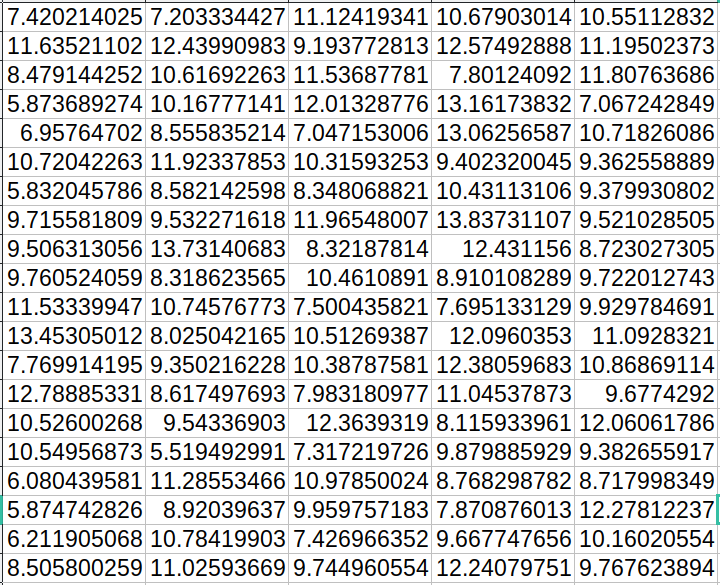
\includegraphics[scale = .35]{Images/100 Samples from Normal.png}
      \caption{For example, this is a sample of 100 points randomly picked from $\mathcal{N}(10, 2^2)$ using a spreadsheet software like Excel.}
  \end{figure}









\end{itemize}
\end{frame}




\subsection{2. Statistical Estimation}
\frame{\subsectionpage}

\begin{frame}[allowframebreaks]{Estimation}
   
\begin{itemize}
   \item Consider the sample again,

      \medskip
      \begin{tabular}{l|c|c|c|c}
      \hline
       & Gender & Monthly Income (tk) & ECO-101 Grade & \# Retakes\\
      \hline
      Student A & Male & 3615 & B- & 3\\
      \hline
      Student B & Female & 49755 & A & 2\\
      \hline
      Student C & Male & 44758 & A & 1\\
      \hline
      Student D & Female & 3879 & B & 0\\
      \hline
      Student E & Male & 22579 & A+ & 2 \\
      \hline
      \end{tabular}



    \item Now again, think about following questions,

    \begin{itemize}
       \item do we know the \alert{population mean of income} from all students, \emph{call it $\mu$?} 

       \medskip

           \emph{Ans - NO, we don't know $\mu$, (Here $\mu$ is just some number which is the population average)}
      \medskip

      \item  Similarly  do we know the \alert{population proportion of all female students}, call it $p$? 

      \medskip
      \emph{Ans - NO (here $p$ is probability)}
      \medskip 


    \end{itemize}



  \item Now can we \emph{estimate}  $\mu$ or $p$? Ans: Yes - we can use our sample to \emph{estimate}. 

  \item For example, \alert{sample mean of income}, denote this with $\bar{x}$ can be used to estimate $\mu$. For example here $\bar{x} = 124586$ (Just simply take the average). This is the \emph{estimate of the population mean $\mu$}.

  \item Similarly \alert{sample proportion of female students}, call it $\bar{p}$ can be used to estimate population proportion $p$. Here if we think Female = 1, and Male = 0, and then sample proportion is $\bar{p} = 0.4$ (Just simply take the average). This is the \emph{estimate of the population proportion $p$}.


  \item This is the idea of \emph{Estimation}, that is

  \medskip
  \alert{there is a target parameter for example $\mu$ or $p$, which is a population object, but we don't know it, then we will estimate these objects with some numbers using a sample}.
  \medskip

  \item The number that we calculate using a sample is called \emph{an estimate}.

  \item Now \emph{does our estimate get better if we increase the size of the sample (or sample size $n$)}? 

  \item The answer is Yes - if we have a good sample and we increase the sample size then maybe we expect that we will \alert{eventually be very very close to the target parameter!}

  \item What happens if we get a bad sample? Then even if we increase the sample size, our estimate won't improve.

  \item There is a famous saying in Statistics, \alert{Garbage in Garbage out!} This means if you have a bad sample, then even if you increase the sample size, you will not get a good estimate. 


  \framebreak

  \item But if we have a good sample, there is a famous law in Statistics, called \alert{Law of Large Numbers}, this says if we increase the sample size, then our estimate will get better and better and we will eventually hit the target parameter! In notation we can write this as

   \begin{align*}
      \text{if } n \to \infty \text{ then } \bar{x} \to \mu \text{ and this happens with very high probability}
   \end{align*}


   \item This is one of the most important results in Statistics, that is with good samples, we can estimate the target parameter with high accuracy if we have a very large sample. 

   \item This idea is also known as \emph{Consistency} of an estimator, which we will discuss in coming sections.



  \item So again to summarize, this process of targeting something from the population and then guessing that with the help of sample is known as \emph{Estimation} or more accurately this is called \emph{Point Estimation}, it's a concept in Inferential Statistics, but there is another method known as hypothesis testing, we won't cover it here you will see it in the next course.

  \item Both estimation and testing are part of inferential statistics

% \medskip
% \begin{itemize}
%   \item 1. Estimation - Point Estimation and Interval Estimation (a.k.a confidence interval)
%   \item 2. Testing (a.k.a Hypothesis Testing).
% \end{itemize}
% \medskip

% \item Let's write the idea of point estimation using some notation. Suppose we are interested in the \alert{Population mean $\mu$} But we cannot access it and we only have a sample $x_1, x_2, \ldots, x_n$ (These are fixed numbers for a sample of size $n$). So we find the sample mean $\bar{x} = \frac{1}{n} \sum_{i = 1}^{n} x_i$. This sample mean $\bar{x}$ is a \alert{point estimate} of the \alert{unknown Population mean $\mu$}.


\item Question  - \emph{Since we can think the sample is random does this estimate change with different samples}? Ans: obviously YES!

\item How do we write this? We need to think about random variables.... here the idea of \emph{Estimator} comes...

 \framebreak


\item Now let's consider another data, suppose we collected a data from $10$ students, which are just income of $10$ students, and we are interested in the population mean $\mu$.


    \small{
      \begin{table}[H]
      \begin{tabular}{|c|c|c|}
      \hline & Income & Random variable \\
      \hline 1. & 20 & $X_1=?$ \\
      \hline 2. & 60 & $X_2=?$ \\
      \hline 3. & 20 & $X_3=?$ \\
      \hline 4. & -20 & $X_4=?$ \\
      \hline 5. & -30 & $X_5=?$ \\
      \hline 6. & -10 & $X_6=?$ \\
      \hline 7. & 80 & $X_7=?$ \\
      \hline 8. & 10 & $X_8=?$ \\
      \hline 9. & 30 & $X_9=?$ \\
      \hline 10. & 40 & $X_{10}=?$ \\
      \hline
      \end{tabular}
      \caption{Income data}
      \end{table}
    }


\item As you probably already know, a data set can be thought in two ways, a fixed data or a random data. 

\item Note in the left column we have fixed data, but in the right column we have random variables. So  $X_1$ is a random variable, $X_2$ is a random variable, $\ldots$, $X_{10}$ is a random variable. Important is in the case of  \emph{realized data / fixed data},  the randomness is gone and we have observed the value.





 \item Generally  when we think about $n$ random variables,  $X_1, X_2, X_3, \ldots, X_{n}$, we will call it a \emph{random sample} (the other one is the fixed sample!)

 \item Now we will talk about Estimator. 

 \item The idea of \emph{Estimator} comes when we think about a random sample. An Estimator is a \emph{function of a random sample}, hence this is also a \emph{random variable}. For example an estimator of $\mu$ is 

  \begin{align*}
    \bar{X} &= f(X_1, X_2, \ldots, X_n) = \frac{1}{n}\sum_{i = 1}^{n} X_i
  \end{align*}

  \item Now this is not just ordinary sample mean. This is a random variable, since it's a function of random variables $X_1, X_2, \ldots, X_n$. It's value will change from sample to sample ....


  \item So now you should always remember the difference between $\bar{x}$ and $\bar{X}$. For a fixed sample $\bar{x}$ is a fixed number, but $\bar{X}$ is a random variable. This is random since it changes from sample to sample. But again, when we calculate it for a fixed sample, then we get a fixed number $\bar{x}$. Here $\bar{x}$ is a constant and it's not random.

  \item So the random variable $\bar{X}$ is an estimator of $\mu$. And the fixed number $\bar{x}$ is an estimate of $\mu$.



  \item  Now since $ \bar{X}$ is a random variable, question is what is the probability distribution of $\bar{X} $? or Expectation of $\mathbb{E}(\bar{X})$? Or $\Var(\bar{X})$

\item To understand this we need to talk abut the sampling distribution of $\bar{X}$, which we will do in the next section.


 
\end{itemize}

\end{frame}


\section{Sampling Distributions}
\frame{\sectionpage}


%-----------------------------------------------------------------------------


\subsection{Mean and Variance of $\bar{X}$}
\frame{\subsectionpage}
\begin{frame}[allowframebreaks]{Estimator $\bar{X}$, $\mathbb{E}(\bar{X})$ and $\Var(\bar{X})$}



\begin{itemize}
  \item Before we dive with the sampling distribution, let's talk about the estimator $\bar{X}$, and it's mean and variance. When it comes to $\bar{X}$ we are interested in 3 important questions when it comes to estimator,

  \medskip


    \item[1.] What is the Expectation of the random variable $ \bar{X}$, written as $\mathbb{E}(\bar{X})$? 
    \item[2.] What is the variance of the random variable $ \bar{X}$, written $\Var(\bar{X})$?
    \item[3.] What is the probability distribution of $ \bar{X}$ (this is what we call \emph{sampling distribution of $ \bar{X}$ !})


  \framebreak

  \item We are interested in the first question since we want to know how our estimates (for example sample means) performs on average. For example the crucial question here is whether we have $\mathbb{E}( \bar{X})$ becomes close to $\mu$. 


  \item The answer of the second question tells us how much variability we have in our estimates. For example if we have $\Var(\bar{X})$ is small, then we know that our estimate is always close to $\mu$ (this is good!). But if we have $\Var(\bar{X})$ is large, then we know that our estimate is not always close to $\mu$ (this is a bad!)


  \item The answer to the third question is what we call \emph{Sampling Distribution of Sample Means}. Note that, this is the distribution of sample means $\bar{x}$, that we get from repeated sampling!


  \item Definitely if we know the answer of $3$, we know the answers of $1$ and $2$.

  \item Let's try to understand with the following picture. Suppose we do sampling many times and calculate $\bar{x}$ many times, here are four situations that can happen, at the center we have $\mu$ and the black dots are the estimates $\bar{x}$ for different samples.


\framebreak

\begin{figure}
\centering
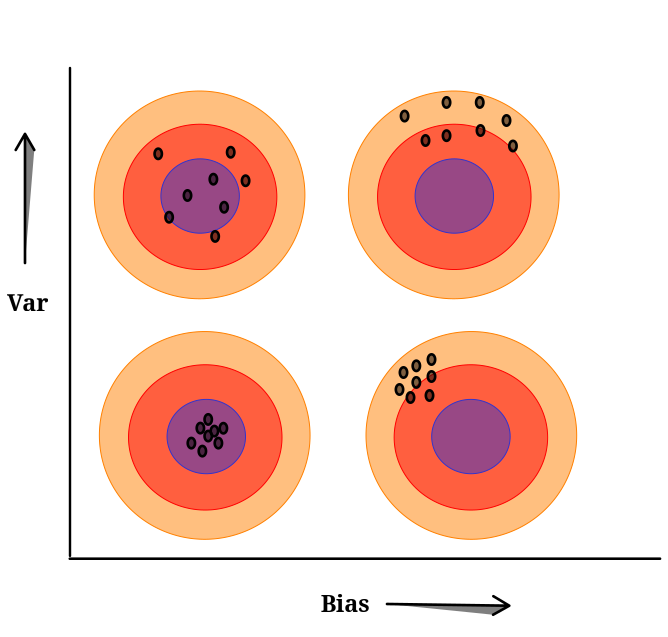
\includegraphics[scale  = .2]{Images/Dart_bias_var.png}
\caption{bias variance situations, true value $\mu$ is at the center, and the black dots are estimates or $\bar{x}$. Here in all four situations think about repeated sampling, i.e., we are calculating $\bar{x}$ in repeated sampling.}
\vspace*{-.4cm}
\end{figure}

\begin{itemize}
\item 1. \emph{top-left:} Here sometimes the estimates are hitting the target, but their accuracy overall is really bad. You can say on average they are performing well, but there is a lot of variability. This is what we call \alert{low-bias \& high-variance} situation.

\item 2. \emph{bottom-left:} This is better than the last one (in fact this is the best one) here estimates are always very close to the truth and also the variability is very low. This is what is called \alert{low-bias \& low-variance} situation. This is ideally what we want.

\item 3. \emph{bottom-right:} In this case the variability is not high, but the estimates are more or less always very off from the target. This is called \alert{high-bias \& low-variance} situation. This is not good, even if we have low variance.

\item 4. \emph{top-right:} This is the worst case, here the estimates are always very off from the target and also the variability is very high. This is called \alert{high-bias \& high-variance} situation.
\end{itemize}


  \item Definitely we want 

    \begin{align*}
    \mathbb{E}(\bar{X}) = \mu
  \end{align*}

  \item If this happens we call $\bar{X}$ an ``unbiased'' estimator of $\mu$. It means the sample average is a ``good'' estimator for the population mean $\mu$. So you can think - if we calculate, sample means many times, \emph{on average} we are not doing a bad job, even if our sample size $n$ is not that big.

  \begin{align*}
    \mathbb{E}(\bar{X}) = \mu
  \end{align*}


  \item Compare this with consistency!

  \item Now let's talk about the sampling distribution of $\bar{X}$. This is the distribution of $\bar{X}$ when we do repeated sampling. 



\end{itemize}
\end{frame}









\subsection{Sampling distribution of $\bar{X}$}
\frame{\subsectionpage}

\begin{frame}[allowframebreaks]{Estimator $\bar{X}$, $\mathbb{E}(\bar{X})$ and $\Var(\bar{X})$}



\begin{itemize}

\item We will state three important results, related to the sampling distribution of $\bar{X}$.



    \begin{varblock}{\Thm{Theorem~} (Mean and Variance of $\bar{X}$ with only i.i.d assumption) }

      Suppose the population distribution have mean $\mu$ and variance $\sigma^2$ and sample points are independent, then

      \begin{align}
          \mathbb{E}\left(\bar{X}\right)  =\mu \text{ and } \mathbb{V}\mathrm{ar}\left(\bar{X}\right)  =\frac{\sigma^2}{n}
      \end{align}

  \end{varblock}

    \item How do we get this? The proof is very simple, just uses the rule for Expectation and Variance. First let's understand the result and then we will also see how we got this,


\framebreak

  \item Note that, in this result \emph{we don't have any distributional assumption} (i.e., we are not assuming they are normal or binomial or anything else...), we are assuming that the population mean and variance exists and we have i.i.d sample points. 


  \item If we think about $X_1, X_2, \ldots, X_n$ random variable this means we have independent and identically distributed random variables (i.i.d)  with the same mean $\mu$ and same variance $\sigma^2$. Again to explain further, this means

  \begin{itemize}
    \item[1.]   $X_1, X_2, \ldots, X_n$  random variables are independent, 
    \item[2.] $X_1, X_2, \ldots, X_n$  have same probability distribution where we have $\mathbb{E}(X_1) = \mathbb{E}(X_2) = \mathbb{E}(X_3) = \ldots, \mathbb{E}(X_n) = \mu$, and also $\Var(X_1) = \Var(X_2) = \Var(X_3) = \ldots, \Var(X_n) = \sigma^2$
  \end{itemize}

  \item Finally you should always keep in mind that $\bar{X}$ is a random variable, since it's a function of random variables $X_1, X_2, \ldots, X_n$.

  \item Now let's see the details....




\framebreak




    \item We know that $\mathbb{E}(X_i) = \mu$ and $\Var(X_i) = \sigma^2$, then we can apply the rules for expectation and variance.


    \begin{align*}
        \mathbb{E}(\bar{X}) &= \mathbb{E}\left(\frac{1}{n} \sum_{i = 1}^{n} X_i\right) = \frac{1}{n} \sum_{i = 1}^{n} \mathbb{E}(X_i) = \frac{1}{n} \sum_{i = 1}^{n} \mu = \frac{n \times \mu}{n} = \mu 
    \end{align*}

    \begin{align*}
        \Var(\bar{X}) &= \Var{\left(\frac{1}{n} \sum_{i = 1}^{n} X_i \right)} \overset{*}{=} \frac{1}{n^2} \sum_{i = 1}^{n} \Var(X_i) = \frac{1}{n^2} \sum_{i = 1}^{n} \sigma^2 =  \frac{n \times \sigma^2}{n^2}  = \frac{\sigma^2}{n}
    \end{align*}

    \item For expectation this is simply the rule for expectation - Expectation of sum of independent random variables is the sum of expectation of each random variable. 


    \item For the variance we used the fact that $X_i$'s are independent, so we can apply the rule for variance for the sum of independent random variables. In particular we used the fact that 

    \begin{align*}
        \Var(X_1 + X_2) = \Var(X_1) + \Var(X_2) \text{ if $X_1$ and $X_2$ are independent }
    \end{align*}

    \item Finally we also used the fact that $\Var(aX) = a^2 \Var(X)$ for any constant $a$.


    \framebreak

    \item Careful if they are not independent then this is not true! we will have 

    \begin{align*}
          \Var{(X_1 + X_2)} = \Var{(X_1)} + \Var{(X_2)} + 2 \mathbb{C}\mathrm{ov}(X_1, X_2)
    \end{align*}
    
    \item When we have independence, covariance is zero, so we get 

        \begin{align*}
          \Var(X_1 + X_2) &= \Var(X_1) + \Var(X_2) + 2 \underbrace{\mathbb{C}\mathrm{ov}(X_1, X_2)}_{=0} \\
          &= \Var(X_1) + \Var(X_2) 
    \end{align*}






\framebreak



\begin{varblock}{\Thm{Theorem~} (Distribution of $\bar{X}$ with Normality and i.i.d assumption) }

If the \emph{population distribution is $\mathcal{N}(\mu, \sigma^2)$} (this means population is normally distributed with mean $\mu$ and variance $\sigma^2$) and the sample points are independent, then 

\begin{align}
  i) &\quad \mathbb{E}\left(\bar{X}\right)  =\mu \text{ and }  \Var{\left(\bar{X}\right)  =\frac{\sigma^2}{n}} [\text{ this is same as the last one }] \nonumber\\
 ii) &\quad \bar{X} \sim \mathcal{N}(\mu, \frac{\sigma^2}{n})  \text{ from transformation }  Z \sim \mathcal{N}(0, 1) \text{ where } Z = \frac{ \bar{X}  - \mu}{\cfrac{\sigma}{\sqrt{n}}}
 \nonumber\\
  iii) &\quad t \sim t_{n-1} \text{ where } t = \frac{ \bar{X}  - \mu}{\cfrac{S}{\sqrt{n}}} \text{ and } S^{2} = \frac{1}{n-1} \sum_{i=1}^{n} (X_i - \bar{X})^2 \nonumber
\end{align}

\end{varblock}


  \item  {\color{red} Careful} Here $ S^{2} = \frac{1}{n-1} \sum_{i=1}^{n} (X_i - \bar{X})^2$ is sample variance but we are thinking it as a random variable (so its value changes in repeated sampling). This makes $t$ a random variable which is a function of random variables $\bar{X}$ and $S$. 

  \item Number $iii)$ says if we replace $\sigma$ with $S$ (this means replacing population standard deviation with sample standard deviation), we get a new random variable $t$, which follows $t$ distribution with $n-1$ degrees of freedom. This is called \emph{Student's t-distribution}. 

  \item Here $n- 1$ is the parameter of the $t$ distribution. This parameter has a special name, it is called \emph{degrees of freedom}. 



  \item Also note here $\bar{X}$ is a statistic, $Z$ is a statistic and also $t = \frac{\bar{X} - \mu}{S / \sqrt{n}} $ is a statistic (Recall a statistic is a function of a random sample). 

  \item In practical cases we don't know the population standard deviation $\sigma$, so we use the sample standard deviation $S$ to estimate $\sigma$. Since $\sqrt{\Var(\bar{X})} = \frac{\sigma}{\sqrt{n}}$, is the \emph{standard error} of the sample mean $\bar{X}$. $S / \sqrt{n}$ is called the \emph{estimate of the standard error of the sample mean}.


  \item Note that this result assumes stronger assumption than the last one, we are assuming population is normal.

  \item The next theorem will relax this assumption but we will need large $n$.

  % \item The next theorem is also one of the most important results in Statistics, this is called \emph{Central Limit Theorem (CLT)}. Roughly speaking this says if we have a large sample size, then the distribution of $\bar{X}$ will be approximately normal. 



  \framebreak




 


\begin{varblock}{\Thm{Theorem~} (Central Limit Theorem (CLT) and related results) }

  Let $X_1, X_2, \ldots, X_n$ be i.i.d random variables that follow \alert{any distribution} with population mean $\mu$ and variance $\sigma^2$. Then for \emph{large $n$ (technically we need $n \to \infty$)}, we get following results:

      \begin{align}
          &i)\quad  Z \overset{approx}{\sim} \mathcal{N}\left(0, 1\right)  \text{ where } Z = \frac{ \bar{X}  - \mu}{\cfrac{\sigma}{\sqrt{n}}} \quad \text{ \color{red}[CLT] } \\ \nonumber 
          &ii)\quad  \bar{X} \overset{approx}{\sim} \mathcal{N}\left(\mu, \frac{\sigma^2}{n}\right)\\ \nonumber 
          &iii)\quad t \overset{approx}{\sim} \mathcal{N}\left(0, 1\right)   \text{ where } t = \frac{ \bar{X}  - \mu}{\cfrac{S}{\sqrt{n}}} \nonumber 
      \end{align}

  \end{varblock}


\item This is one of the most important results in Statistics. This is called \emph{Central Limit Theorem (CLT)}. This says if we have a large sample size, then the distribution of $\bar{X}$ will be approximately normal. 

\item i) says without any distributional assumption the $Z$ statistic will be approximately normal in large samples.

\item ii) says the sample mean $\bar{X}$ will be approximately normal in large samples.


\item iii) says the $T$ statistic will be approximately normal in large samples. You should compare this $T$ with $t$ in Theorem 5.3 iii). Both are same, so in calculation there is no difference but in assumptions there is a big difference. In Theorem 5.3 iii) we are assuming the population is normal, but here we are not assuming anything about the population. In that case $t$ statistic follows $t$ distribution, but here the sane statistic $T$ follows normal distribution in large samples. 






\end{itemize}




\end{frame}

%-----------------------------------------------------------------------------


\begin{frame}[allowframebreaks]{Important Remarks on Sampling Distribution of $\bar{X}$}

  
\begin{itemize}
  \item So we understood that \emph{the idea of the sampling distribution is a repeated sampling idea}. In real life you can only have one sample, so you can never calculate this using a sample data.

  \item The last three results tell us that, we can only know the sampling distribution of means under certain assumptions (in particular we need either normality or large sample size)

  \item If we assume normality (this means our data is normally distributed), then the distribution of the sample means is also normal and this result is for any sample size! This is called the \emph{exact distribution}!

  \item If we don't assume normality for the population, then usually we have no hope, except for large $n$.
  
  \item The standard deviation of sampling distribution is called \emph{standard error}! This is standard deviation, but this name is special for sampling distribution.


  \item In general \emph{any function} of the random sample $X_1, X_2, \ldots, X_n$ is called a ``\emph{Statistic}'', so an estimator is also a \alert{Statistic}. The difference is Estimator is a type of Statistic where we are estimating some target! A statistic might not have any goal, it's just a function of random variables $X_1, X_2, X_3, \ldots, X_n$! The distribution of statistic is called \emph{sampling distribution}. 

  \item For example, $\bar{X}$, $Z$ in Theorem 5.3 are both examples statistics but $\bar{X}$ is an estimator for $\mu$, $Z $ is just a statistic.

  \item Another example is $S^2$, where $S^2=\frac{1}{n-1} \sum_{i=1}^n\left(X_i-\bar{X}\right)^2$. This is  a statistic since it's a function of the random sample. And this is also an estimator for $\sigma^2$, because it is targeting population variance $\sigma^2$. Note that $S^2$ is just a sample variance.




\end{itemize}

\end{frame}



\subsection{Sampling Distribution of Sample Proportions, i.e., Sampling distribution of $\bar{p}$}
\frame{\subsectionpage}

\begin{frame}[allowframebreaks]{Sampling Distribution of $\bar{p}$}
  
  \begin{itemize}
  \item Sampling distribution of sample proportion is just a special case of sampling distribution of sample means, except now we are considering \emph{sample mean of Bernoulli random variables.} 

  \item Let's first think \emph{what is a population proportion?} Suppose we have a large population and there are certain proportions of females in this population, let's call this number $p$. This is the population proportion. Now we can think about taking a sample of size $10$ from this population such that all the rows are independent. 

        \begin{table}[H]
      \begin{tabular}{|c|c|c|}
      \hline & Income & Random variable \\
      \hline 1. & 1 & $X_1=?$ \\
      \hline 2. & 1 & $X_2=?$ \\
      \hline 3. & 0 & $X_3=?$ \\
      \hline 4. & 0 & $X_4=?$ \\
      \hline 5. & 1 & $X_5=?$ \\
      \hline 6. & 0 & $X_6=?$ \\
      \hline 7. & 1 & $X_7=?$ \\
      \hline 8. & 0 & $X_8=?$ \\
      \hline 9. & 1 & $X_9=?$ \\
      \hline 10. & 1 & $X_{10}=?$ \\
      \hline
      \end{tabular}
      \caption{Income data}
      \end{table}

    \item Here $1$ means Female and $0$ means male. Again like before the left column is the observed/realized sample and in the right column we are thinking in terms of random variable $X_1, X_2, X_3, \ldots, X_n$

    \item In this case we can think the random variables $X_1, X_2, X_3, \ldots, X_n$ are all distributed as Bernoulli distribution with parameter $p$, in other words we have 

    \begin{align*}
      X_i \sim \mathrm{Ber}(p) \text{ for all } i = 1, 2, 3, \ldots, n
     \end{align*}

     \item Now we can think about an \emph{estimator for population proportion $p$}

        \begin{align*}
        \bar{p} = \frac{1}{n} \sum_{i = 1}^{n} X_i
        \end{align*}

    \item This is an estimator because for a fixed sample, $\bar{p}$ is a fixed number, but for a random sample $\bar{p}$ is a random variable. 

    \item Now let's apply Theorem 5.2 and 5.3. Since  by assumption $X_1, X_2, X_3, \ldots, X_n$ are all independent and they all follow Bernoulli distribution with parameter $p$, we have

    \begin{align*}
      \mathbb{E}(\bar{p}) = p \text{ and } \Var(\bar{p}) = \frac{p(1-p)}{n}
    \end{align*}


    \item How do we get this? Same as before, note that here 


    \begin{align*}
         \mathbb{E}(X_i) = p \text{ and } \Var(X_i) = p(1-p) \text{ for } i = 1, 2,\ldots, n
    \end{align*}
   
    then applying the rules for expectation and variance, we get


    \begin{align*}
        \mathbb{E}(\bar{p}) &= \mathbb{E}\left(\frac{1}{n} \sum_{i = 1}^{n} X_i\right) = \frac{1}{n} \sum_{i = 1}^{n} \mathbb{E}(X_i) = \frac{1}{n} \sum_{i = 1}^{n} p = p
    \end{align*}

    \begin{align*}
        \Var(\bar{p}) &= \Var{\left(\frac{1}{n} \sum_{i = 1}^{n} X_i \right)} \overset{*}{=} \frac{1}{n^2} \sum_{i = 1}^{n} \Var(X_i) = \frac{1}{n^2} \sum_{i = 1}^{n} p(1-p) = \frac{p(1-p)}{n}
    \end{align*}


    \item So we know that 

    \begin{align*}
      \mathbb{E}(\bar{p}) = p \text{ and } \Var(\bar{p}) = \frac{p(1-p)}{n}
    \end{align*}

    \item Now let's talk about the sampling distribution of $\bar{p}$. In this case we can apply Theorem 5.4 i), which is a large sample result without any distributional assumption, so we get


    \begin{align*}
           \bar{p} \sim \mathcal{N}\left(p, \frac{p(1-p)}{n}\right) \text{ also using transformation } Z \sim \mathcal{N}(0, 1), \text{ where } Z = \frac{\bar{p} - p}{\sqrt{\frac{p(1-p)}{n}}}
    \end{align*}

    \item Here $\sqrt{\frac{p(1-p)}{n}}$ is the \emph{standard error} of $\bar{p}$, or you can say this is the standard deviation of the sampling distribution of $\bar{p}$.


    \framebreak

    \item Now the issue with the $Z$ statistic is that we don't know the population proportion $p$. So we can't use $Z$ statistic in practice, solution? use the sample proportion $\bar{p}$ to estimate $p$, and then construct the $t$ statistic. 

    \item In his case we can apply Theorem 5.4 iii), which is a large sample result without any distributional assumption and also without assuming we know $p$, so we can form the $t$ statistic


    \begin{align*}
      T =  \frac{\bar{p} - p}{\sqrt{\frac{\bar{p}(1-\bar{p})}{n}}} \sim \mathcal{N}(0, 1)
    \end{align*}

    \item You should compare this with the $t$ statistic in Theorem 5.4 (iii), this is exactly same, now we are using $\bar{p}$ instead of $\bar{X}$, and we are using $\sqrt{\bar{p}(1-\bar{p})}$ instead of $S$.


    \item In ECO204 you will see $t$ statistic many times, and all of them will follow the same structure, 

    \begin{align*}
        t = \frac{\text{estimator} - \mathbb{E}\left(\text{estimator}\right)}{\left(\text{estimate of the standard error}\right)}
    \end{align*}

    \item And often in large samples (at least the cases that you will encounter), the distribution of the $t$ statistic will become standard normal. Hence we can use the standard normal distribution to calculate the probability of the $t$ statistic. 


    \item More on this on ECO204...



















\end{itemize}

\end{frame}






\begin{frame}[allowframebreaks]{References}
\vspace*{.3cm} 

\scriptsize
% \printbibliography[maxnames=99]

% \nocite{*}
\bibliographystyle{apalike}
\bibliography{../common/references}  
% \nocite{*}

\end{frame}

\end{document}
